% Chapter 5

\chapter{Déroulement et apports du stage} % 5th chapter title

\label{Chapter5} % For referencing the chapter elsewhere, use \ref{Chapter5} 

%1----------------------------------------------------------------------------------------






\section{Journal de bord}

Le stage s'est déroulé de facon agile. Chaque semaine, un rapport d'activité fur rédigé. Dans ce dernier figurait principalement le travail effectué, les difficultés rencontrées, et le travail à venir durant le nouvelle semaine a venir. Dans cette section, nous résumons le travail effectué durant chacune de ces 26 semaines. Pour des rapports détaillés, le lecteur est invité à se rendre sur le dépot \href{https://github.com/desmond-rn/ice-floes/tree/master/reports/weeks}{ice-floes}.

\paragraph{Semaine 1 (\DTMdisplaydate{2021}{2}{3}{-1} - \DTMdisplaydate{2021}{2}{9}{-1})} 
\begin{enumerate}
    \item Mise en place du \href{https://github.com/desmond-rn/ice-floes}{dépot GutHub} \textbf{privé} pour le suivi de la rédaction des différents documents et le travail à distance plus aisé; 
    \item Lecture de l'article de M. Rabatel et al. \parencite{rabatel2015dynamics}
    \item Lecture de la thèse de M. Rabatel \parencite{rabatel2015thesis} (introduction, chapitres 1 et 2):
    \item Apprentissage et utilisation des principales fonctionnalités du module TikZ.   
\end{enumerate}
  
\paragraph{Semaine 2 (\DTMdisplaydate{2021}{2}{10}{-1} - \DTMdisplaydate{2021}{2}{16}{-1})} 
\begin{enumerate}
    \item Fin de lecture des chapitres 2 et 3 de la thèse de M. Rabatel \parencite{rabatel2015thesis}.
    \item Début de lecture de la thèse de D. Balasoiu \parencite{balasoiu2020thesis}.
    \item Continuation de rédaction de l'état de l'art pour le rapport de stage.
  \end{enumerate}
  

\paragraph{Semaine 3 (\DTMdisplaydate{2021}{2}{17}{-1} - \DTMdisplaydate{2021}{2}{23}{-1})} 
\begin{enumerate}
    \item Révision des notions de mécanique de la rupture (et de mécanique du solide) à travers le livre \parencite{gross2017fracture}.
    \item Lecture de la première partie de la thèse de D. Balasoiu \parencite{balasoiu2020halthesis}).
    \item Début de lecture de la deuxième partie (chapitre 3) \parencite{balasoiu2020halthesis}.
\end{enumerate}
  

\paragraph{Semaine 4 (\DTMdisplaydate{2021}{2}{24}{-1} - \DTMdisplaydate{2021}{3}{2}{-1})} 
\begin{enumerate}
  \item Lecture du chapitre 3, et démonstration de la proposition 3.3.1 \parencite[p.93]{balasoiu2020halthesis}.
  \item Lecture des annexes et relecture (rapide) des chapitres 1 et 2 de la thèse \parencite{balasoiu2020halthesis}.
  \item Lecture du chapitre 4 (sans vraiment comprendre). Des outils avancés de \textbf{théorie de la mesure}, de \textbf{probabilité appliquée}, de \textbf{géométrie stochastique}, \textbf{etc}. sont nécessaires pour comprendre.
  \item Lecture du chapitre 1 du livre \parencite{chiu2013stochastic} cité à plusieurs reprises dans le chapitre 4 de la thèse \parencite{balasoiu2020halthesis}. 
\end{enumerate}

\paragraph{Semaine 5 (\DTMdisplaydate{2021}{3}{3}{-1} - \DTMdisplaydate{2021}{3}{9}{-1})} 
\begin{enumerate}
    \item Réessaie de lecture du chapitre 4 du livre \parencite{balasoiu2020halthesis}.
    \item Lecture du chapitre 2 du livre \parencite{chiu2013stochastic}.
    \item Révisions de notions de théorie de la mesure : \textbf{mesure et formules de Campbell}, \textbf{distribution de Palm}, etc.
    \item Lecture des chapitres 5 et 6 de la thèse \parencite{balasoiu2020halthesis}.
\end{enumerate}
  

\paragraph{Semaine 6 (\DTMdisplaydate{2021}{3}{10}{-1} - \DTMdisplaydate{2021}{3}{16}{-1})} 
\begin{enumerate}
    \item Lecture approfondie des chapitres 4 et 5 du livre \parencite{balasoiu2020halthesis};
    \item Rédaction de l'\/état de l'\/art dans le rapport de stage. 
\end{enumerate}
  

\paragraph{Semaine 7 (\DTMdisplaydate{2021}{3}{17}{-1} - \DTMdisplaydate{2021}{3}{23}{-1})} 

\begin{enumerate}
    \item Test et debuggage du code \verb|spingslattice| sur \href{https://framagit.org/RaK/SimuRessorts}{Framagit}. 
    \item Étude de l'état de l'art pour des problèmes de collision utilisant des réseaux de ressorts \parencite{islam2020numerical,gerivani2019proposing,homodeling,manea2021simplified}.
    \item Relecture de la section 1.1.2 du chapitre 1 de la thèse de \citeauthor{rabatel2015thesis} \parencite[p.18]{rabatel2015thesis}, et proposition d'un problèmes lineaires de complémentarité pour modéliser la collision singulière.
  \end{enumerate}


\paragraph{Semaine 8 (\DTMdisplaydate{2021}{3}{24}{-1} - \DTMdisplaydate{2021}{3}{30}{-1})} 
\begin{enumerate}
    \item Relecture des parties importantes pour la modélisation dans les thèses \parencite{balasoiu2020halthesis,rabatel2015thesis};
    \item Lecture de travaux ayant trait au contact ponctuel entre deux solides (par exemple \parencite{lotstedt1981coulomb}, etc.);
    \item Développement du modèle de percussion et essaies de résolution analytique. 
\end{enumerate}
  

\paragraph{Semaine 9 (\DTMdisplaydate{2021}{3}{31}{-1} - \DTMdisplaydate{2021}{4}{06}{-1})} 
\begin{enumerate}
    \item Lecture de plusieurs modèles de systèmes masses-ressorts avec dispositifs visqueux, en particulier dans \parencite{homodeling}.
    \item Posage du porblème de percission 1D, et d'écrire les équations régissant le système.
    \item Simulation du modèle à l'aide des librairies \verb|Scipy| et \verb|Bokeh| (la simulation interactive a permis de constater des erreurs dans le modèle qui ont aussitot été corrigées). 
\end{enumerate}
  

\paragraph{Semaine 10 (\DTMdisplaydate{2021}{4}{07}{-1} - \DTMdisplaydate{2021}{4}{13}{-1})} 
\begin{enumerate}
    \item J'ai modélisé le contact avec séparaƟon, tout en simulant les différents systèmes 1D décrits dans \emph{Percussion1D-3.ipynb}. 
    \item Preuve des questions d'existence, d'unicité, etc. par rapport au modèle développé.
\end{enumerate}


\paragraph{Semaine 11 (\DTMdisplaydate{2021}{4}{13}{-1} - \DTMdisplaydate{2021}{4}{20}{-1})} 
\begin{enumerate}
    \item La principale tâche effectuée à été l'animation du modèle de percussion 1D. J'ai divisé cette partie en deux phase:
    \begin{itemize}
        \item \textbf{Avant le contact}: pour faciliter les travaux, on suppose que les floes sont en mouvement rectilignes uniformes.
        \item \textbf{Après le contact}: la semaine dernière, nous avons calculé les "vitesses initiales" pour cette phase. On les utilise pour simuler le déplacement.
    \end{itemize}
\end{enumerate}


\paragraph{Semaine 12 (\DTMdisplaydate{2021}{4}{21}{-1} - \DTMdisplaydate{2021}{4}{27}{-1})} 
\begin{enumerate}
    \item Démonstration de la non-convergence du modèle 1D; 
    Une trigonalisation de la matrice du système permet d'exhiber l'expression explicite des déplacements, et de conclure.
    \item Initialisation de la modélisation et de la simulation du modèle 2D.
  \end{enumerate}
  
\paragraph{Semaine 13 (\DTMdisplaydate{2021}{4}{28}{-1} - \DTMdisplaydate{2021}{5}{4}{-1})} 
\begin{enumerate}
    \item Vérification du modèle et du code de calcul 2D. Etude des paramètres et du système masse-ressort en Python.
    \item Relecture du code et la thèse de Dimitri afin de trouver des nouvelles idées.
\end{enumerate}


\paragraph{Semaine 14 (\DTMdisplaydate{2021}{5}{5}{-1} - \DTMdisplaydate{2021}{5}{11}{-1})} 
\begin{enumerate}
    \item Lecture détaillée du code de Dimitri; compréhension des fonction et demande d'aide lorsque nécessaire.
    \item Développement d'un modèle de percussion en 2D compatible avec le code préexistant.
    \item Début d'écriture d'une présentation Beamer pour la soutenance de mi-stage.
\end{enumerate}
  

\paragraph{Semaine 15 (\DTMdisplaydate{2021}{5}{12}{-1} - \DTMdisplaydate{2021}{5}{18}{-1})} 
\begin{enumerate}
    \item Fin de l'écriture de la présentation Beamer pour la soutenance de mi-stage. Modification et incorporation des différentes remarques de M. Labbé. 
    \item Suite de la lecture détaillée du code de Dimitri.
  \end{enumerate}


\paragraph{Semaine 16 (\DTMdisplaydate{2021}{5}{19}{-1} - \DTMdisplaydate{2021}{5}{25}{-1})} 
\begin{enumerate}
    \item Suite de lecture du code de Dimitri, en particulier le module \texttt{Mesh}. J'ai commencé à définir le module \texttt{MultiMesh}, qui représente deux floes en contact. 
    \item Codage de la deuxième phase de la percussion 1D. Les résultats ne sont pas au point, et seront sans doute améliorés dans les semaines à venir.
\end{enumerate}
  

\paragraph{Semaine 17 (\DTMdisplaydate{2021}{5}{26}{-1} - \DTMdisplaydate{2021}{6}{01}{-1})} 
\begin{enumerate}
    \item Finition de l'animation 1D en corrigeant les bugs;
    \item Rédaction du problème de percussion 2D dans le rapport;
    \item Définition et test du maillage \href{https://framagit.org/RaK/SimuRessorts/-/blob/master/springslattice/multimesh.py}{MultiMesh} en vue de la percussion ; et intégration au code de Dimitri.
\end{enumerate}
  

\paragraph{Semaine 18 (\DTMdisplaydate{2021}{6}{02}{-1} - \DTMdisplaydate{2021}{6}{08}{-1})} 
\begin{enumerate}
    \item Début d'implémentation de la classe \href{https://framagit.org/RaK/SimuRessorts/-/blob/master/springslattice/multisolver.py}{MultiSolver} pour gérer la percussion 2D dans le code de Dimitri.
    \item Revisitation de l'animation 1D en distinguant deux cas en fonction des vitesses des floes après le contact.
    \item Étude énergétique pour la validation du système.
    \item Début de l'étude d'une percussion avec plusieurs noeuds par floes (voir \href{https://github.com/desmond-rn/ice-floes/blob/master/code/simu1D/FractureSolver.py}{FractureSolver.py}).
\end{enumerate}
  

\paragraph{Semaine 19 (\DTMdisplaydate{2021}{6}{09}{-1} - \DTMdisplaydate{2021}{6}{15}{-1})} 
\begin{enumerate}
    \item Implémentation du module \href{https://github.com/desmond-rn/ice-floes/blob/master/code/simu1D/FractureSolver.py}{FractureSolver.py} pour la simulation de la percussion.
    \item Migration du code préexistant (depuis les notebook Python) vers le module \texttt{FractureSolver.py} lorsque possible afin d'accélérer le travail.
    \item Étude du coefficient de restitution utilisé en mécanique du contact (voir \parencite[p.21]{acary2004coefficients}).
    \item Étude énergétique pour la validation du nouveau système.
\end{enumerate}
  

\paragraph{Semaine 20 (\DTMdisplaydate{2021}{6}{16}{-1} - \DTMdisplaydate{2021}{6}{22}{-1})} 
\begin{enumerate}
    \item Rédaction du travail de modélisation et de simulation 1D dans le rapport de stage.
    \item Implémentation du module \href{https://framagit.org/RaK/SimuRessorts/-/blob/master/springslattice/multisolver.py}{multisolver.py} et du script \href{https://framagit.org/RaK/SimuRessorts/-/blob/master/percussion-cli.py}{percussion-cli.py} pour la simulation de la percussion 2D. En se servant des code préexistant, on n'a pas à calculer les vitesses après choc. 
\end{enumerate}
  
\paragraph{Semaine 21 (\DTMdisplaydate{2021}{6}{23}{-1} - \DTMdisplaydate{2021}{6}{29}{-1})} 
\begin{enumerate}
    \item Implémentation d'une interface web adaptée au problème de percussion 2D. 
    \item Étude approfondie de l'énergie totale du système en 1D. Après avoir décelé une erreur de quadrature dans mes calculs, j'ai du complètement changer le modèle pour avoir la conservation de l'énergie totale.
    \item Début d'étude du système 1D \emph{à grande raideur}.
\end{enumerate}
  
\paragraph{Semaine 22 (\DTMdisplaydate{2021}{6}{30}{-1} - \DTMdisplaydate{2021}{7}{05}{-1})} 
\begin{enumerate}
    \item Relecture des chapitres 1 et 2 de la thèse de Dimitri, et des parties de la thèse de Mr. Hanen Amor \parencite{amor2008approche}. 
    \item Extraction des déplacements des noeuds de chaque floe impliqués dans la percussion en supprimer le mouvement d'ensemble du floe par comparaison des positions des noeuds à celle du centre de masse du floe.
    \item Étude de la rentabilité d'une fracture suivant le modèle de Griffith.
\end{enumerate}
  
  
\paragraph{Semaine 23 (\DTMdisplaydate{2021}{7}{07}{-1} - \DTMdisplaydate{2021}{7}{13}{-1})} 
\begin{enumerate}
    \item Redesign du code de calcul 1D : en effet, le code préexistant ne traitait que deux floes, alors qu'on veut à présent en traiter potentiellement plusieurs (\emph{à chaque fracture d'un ressort, c'est un nouveau floe de glace qui se forme}).
    \item Début de l'écriture du code avec debuggage et test au fur et a mesure (approche \emph{agile}).
\end{enumerate}


\paragraph{Semaine 24 (\DTMdisplaydate{2021}{7}{14}{-1} - \DTMdisplaydate{2021}{7}{20}{-1})} 
\begin{enumerate}
    \item Suppression des dictionnaires et adoption d'une approche par classes ; ce qui a considérablement accélérer le développement.
    \item Implémentation des différentes fonctions nécessaires pour simuler le déplacement de plus de deux floes 1D simultanément.
\end{enumerate}
  
\paragraph{Semaine 25 (\DTMdisplaydate{2021}{7}{21}{-1} - \DTMdisplaydate{2021}{7}{27}{-1})} 
\begin{enumerate}
    \item Reconception du code. Nous avons dû éliminer la méthode par numéro de confirmation postulée la semaine dernière ;
    \item Simulation de la fracture de deux floes suivant le modèle de Griffith par une approche combinatoire;
    \item Correction de la visualisation des différents floes après percussion et fracture.
\end{enumerate}
  
\paragraph{Semaine 26 (\DTMdisplaydate{2021}{7}{28}{-1} - \DTMdisplaydate{2021}{8}{03}{-1})} 
\begin{enumerate}
    \item Réussite de la simulation de la percussion et de la fracture de plusieurs floes 1D.
    \item Réétude de l'influence du coefficient de restitution $\varepsilon$. En effet, l'nénergie totale (en particulier l'énergie cinétique) ne devrait pas etre conservée pour $\varepsilon \not 1$.
    \item Rédaction de l'introduction du rapport de stage.
\end{enumerate}
  
\paragraph{Semaine 27 (\DTMdisplaydate{2021}{8}{04}{-1} - \DTMdisplaydate{2021}{8}{13}{-1})} 
\begin{enumerate}
    \item Rédaction du corps et de la conclusion pour le rapport de stage;
    \item Génération des plots et écriture des équations à introduire dans le rapport. 
\end{enumerate}

\paragraph{Semaine 28 (\DTMdisplaydate{2021}{8}{14}{-1} - \DTMdisplaydate{2021}{8}{20}{-1})} 
\begin{enumerate}
    \item Incorporation des notes et des remarques de M. Labbé dans le rapport de stage.
    \item Mise à jour de la présentation de mi-stage;
    \item Rédaction de la présentation de soutenance de stage.
\end{enumerate}

\vspace*{0.65cm}
% \paragraph{Résumé}
Pour résumer les taches effectutées et mieux observer le déroulement du stage, nous avons effectué le graphique de la \cref{fig:timeline}. En comparant ce graphique aux objectifs que nous nous somme fixés dans la \cref{sec:introobk}, nous pouvons faire un bilan du travail qui a été fait.

\begin{figure}[!h]
    \centering
    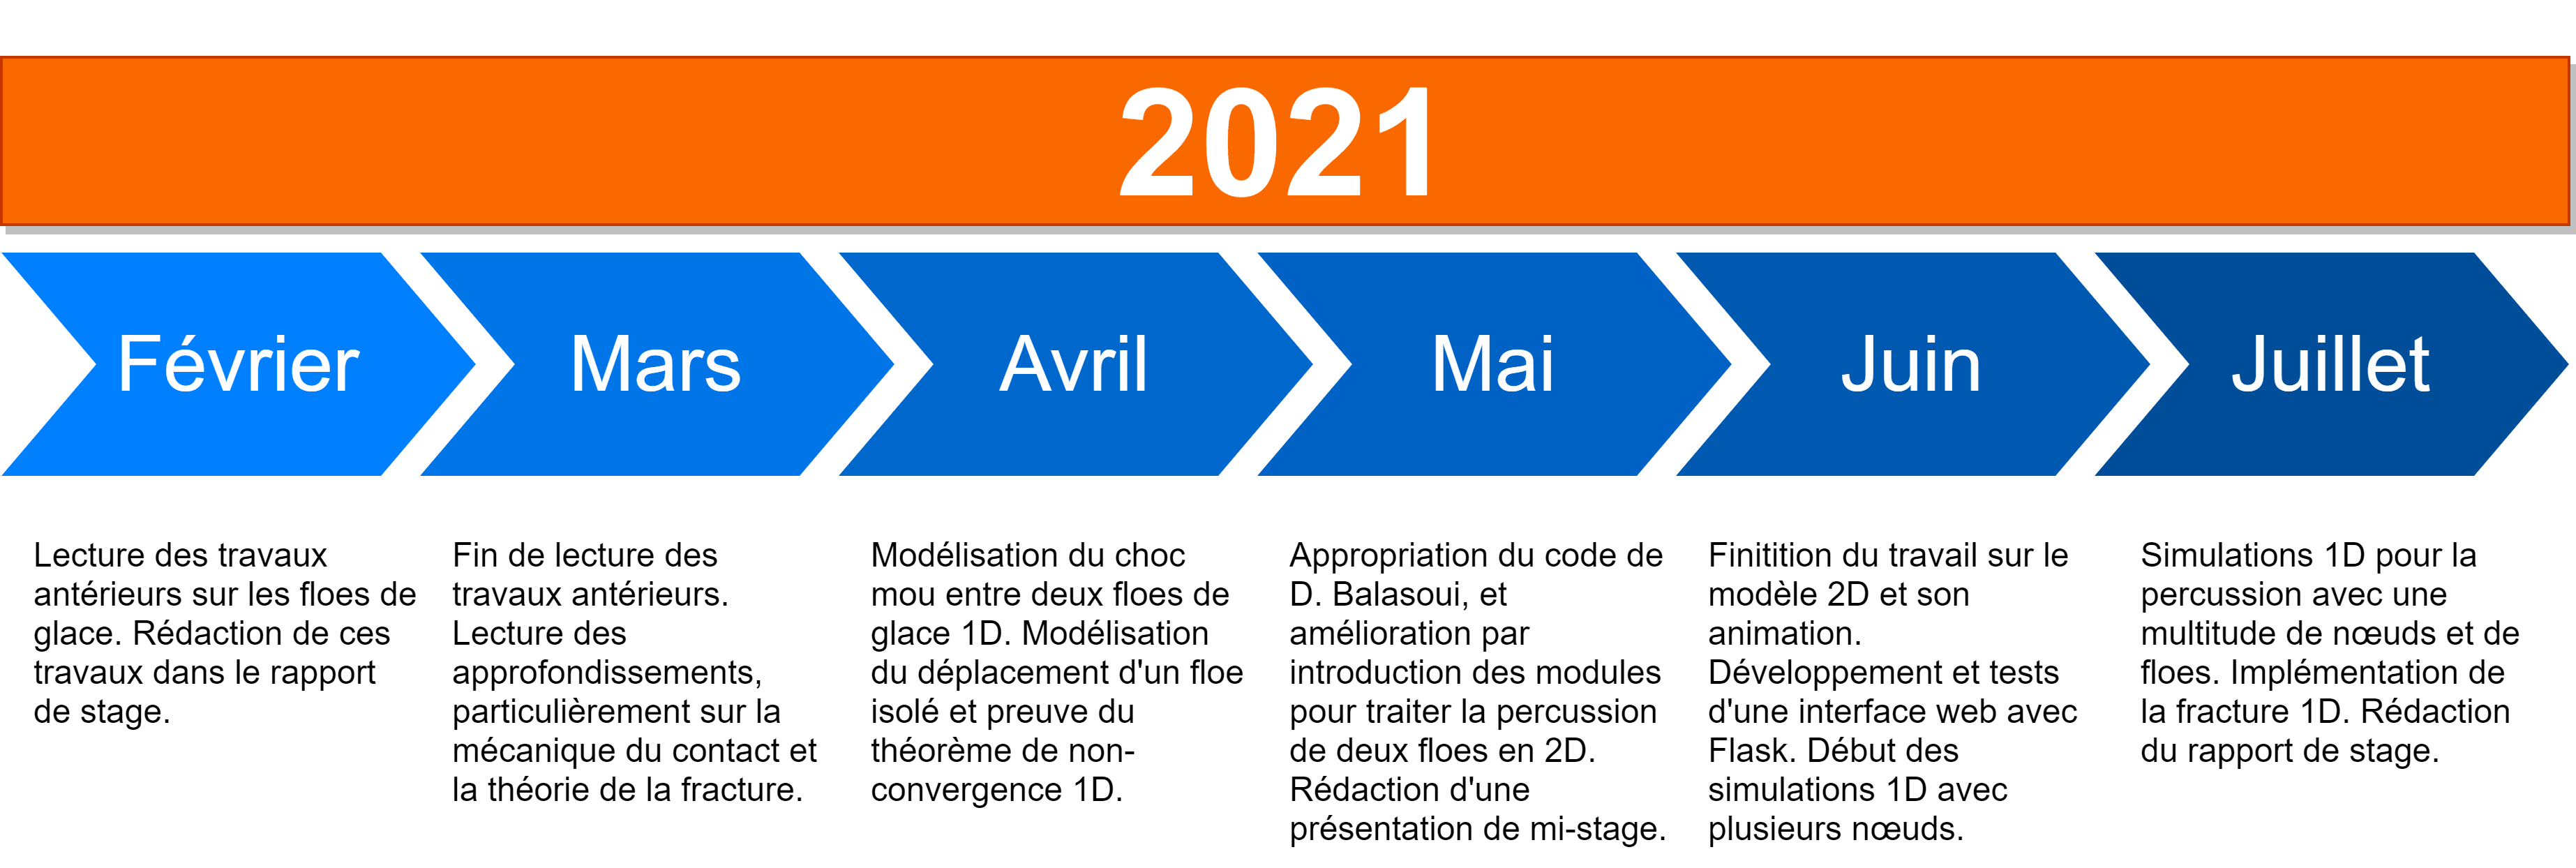
\includegraphics[width=\textwidth]{Timeline.png}
    \caption{Résumé du déroulement du stage.}
    \label{fig:timeline}
\end{figure}


%2----------------------------------------------------------------------------------------






\section{Bilan et future travail}

Durant ce stage, nous avons modéliser et simuler la percussion de floes de glace. Nous avons fait cela en 1 dimension et nous avons convenablement adapté les résultats en simension supérieure, en se servant des travaux précédents sur ce sujet. En plus, nous modélisé et implémenté la fracture en d'un floe de glace 1D. Ceci dit, plusieurs taches restent à effectuer pour porter à fruition notre objectif primaire de creation d'un code de calcul de l’évolution de la banquise à l’échelle des floes de glace:

\begin{itemize}
    \item \textbf{Implémentation de la méthode du champ de phase sue le modèle 1D.} L'approche du champ de phase a longement été présentée à la \cref{subsubsec:approchephase}. Comme nous l'avons indiquée, elle est la mieux adaptée à l'étude de la fracture suivant l'approche variationnel de Francfort et Marigo.
    \item \textbf{Implementation de la fracture au problème 2D.} Durant sa thèse, \citeauthor{balasoiu2020halthesis} a implémenté un modèle quasi-statique de fracture variationnel à travers une méthode éléments finis reposant sur une approche par champ de phase pour régulariser la fracture. Ces travaux sont regroupé dans le dépot sur \texttt{framagit} nommé \href{https://framagit.org/RaK/Griffith}{Griffith}. Il faudra intégré ces travaux au modèle de percussion 2D que nous avons développé durant ce stage.
    \item \textbf{Intégration de la fracture fragile au code de \citeauthor{rabatel2015thesis}.} Comme nous l'avons précisé, \citeauthor{rabatel2015thesis} a, durant sa thèse étudié la dérive d'un ensemble de floes de glace dans la mer. Il faudra donc introduire la fracture de la glace dans ce modèle.
    \item \textbf{Passage en dimension supérieure.} Pour aller plus loin, nous conseillons de passer en trois dimension. Celà dit, les tailles des floes peuvent etre négligeable devant le rayon de la Terre, où la taille de la mer. Il faudra donc prendre celà en considération pour faire des simplifications.
    \item \textbf{Confiramtion de l'approximation par réseaux de ressorts.} D'après la modelisation de Balasoui \parencite{balasoiu2020halthesis}, un assemblage de masses reliées par des ressorts n'est une bonne approximation que si les raiderur on une forte raideur. IL faudra donc augmenter la raideur des ressorts dans les simulations pour observer le comportement des floes, celà permettra d'extraire une deuxième limite spatiale. De plus, Balasoiu a ajouté les dispositifs visqueux pour dissiper les vibrations dans le matériaux. Un futur travail pourrrait donc étudier la nécéssité d'introduire ces dispositifs (qui complexifie considérablement les calculs) dans nos modèles.  
    \item \textbf{Optimiser des codes avec Cython.} En effet, les codes sont écrits en Python durant cette phase . Ce language ne nous permet pour l'instant que d'éfffectuer des simulation avec un nombre restraint de neouds. On pourra donc utiliser \href{https://cython.org/}{Cython} pour faire appel aux fonctions à haute performace du language C. Ou mieux encore, nous pourront reimplémenter tous le code en C$++$ en intégrant les librairies HPC telles que \href{http://www.netlib.org/blas/}{Blas}, \href{https://www.openmp.org/}{OpenMP}, \href{https://developer.nvidia.com/cuda-zone}{CUDA}, etc.
    \item \textbf{Tests de validation en laboratoire.} Des tests en laboratoire sont nécéssaire pour validé les modèles développés. Tout comme \citeauthor{rabatel2015thesis} l'a fait, l'on pourra se servir des données \textbf{ERAinterim} et \textbf{TOPAZ} pour effectuer ces tests.
\end{itemize}






%3----------------------------------------------------------------------------------------




\section{Les apports du stage}


J'ai maitrisé la majeure partie des objectifs que nous nous étions fixés. Cela dit, les apports de ce stages ont été incomptables, et sur plusieurs plans. Tout d'abord sur un plan académique, ou j'ai pris en mains des notions clées des mathématiques appliquées et de l'informatique. Ensuite sur un plan technique, j'ai pu maitriser des outils et faire usage de ressources varirées. Enfin, sur un plan profesionnel ou j'ai pu apprendre d'avantage sur le monde de la recherche.



\subsection{Compétences académique}

\begin{itemize}
    \item \textbf{Simulation de processus physiques:} Ce stage m'a appris à simuler des objects répondant à une loi de comportement bien présice (loi de Newton-Euler, EDO du second ordre) par l'intermédiare de schéma appropriés. Par exmple, un schéma explicite d'ordre 2 pour l'SYSTÈME 2D diverge très fréquement, alors qu'un shéma symplectique (voir \cref{AppendixA}), où un schéma explicite Runge-Kutta d'ordre 4 (RK4) à pas de temps suivant RK5 (comme ceux implémenté par \href{https://docs.scipy.org/doc/scipy/reference/generated/scipy.integrate.solve_ivp.html}{Scipy}) conserve les invariants du système.
    \item \textbf{Prise en main du modèle de rupture de Griffith dans les milieux élastiques:} En lisant les travaux qui ont ptécédé \parencite{balasoiu2020halthesis}, j'ai pu apprendre beacoup sur le modèle de Griffith et la compétition entre les énergie de déformation et de fracture du matériau. J'ai aussi lu les articles \parencite{francfort1998revisiting,bourdin2008variational} et j'ai ainsi assimilé l'approche variationnelle de Francfort, Marigo, Bourdin. Ces notions m'ont poussé à visiter des outils mathématiques très puissant tels que le calcul des variations et la $\Gamma$-convergence (voir \cref{AppendixB}).
    \item \textbf{Maitrise des réseaux de ressorts:} Les travaux de \citeauthor{balasoiu2020halthesis} m'ont également appris comment étudier un matéraux élastiques (réseau de ressorts) par l'intermédiaire d'un processus de poissons \parencite{khasminskii2011stochastic}\footnote{Merci à M. Labbé de m'avoir offert ce livre :)}. J'ai par exmeple appris comment créer (manuellement ou en se servant de la librarie \texttt{Scipy}) un processus de Poinsson répondant à un certain nombre de critères (en particulier l'\emph{intensité}).
    \item \textbf{Développement d'applications en language Python:} Durant ce stage, j'ai énormément améliorer mes compétences en simulation numérique via Python. J'ai par exemple appris comment créer, modifier et déployer un package Python, comment utiliser plusieurs libraries (\texttt{numdifftools}) de calcul scientifique pour mener à bien un projet.
\end{itemize}




\subsection{Compétences techniques}

\begin{itemize}
   \item \textbf{Utilisation de TikZ:} Le premier outils que j'ai maitrisé durant ce stage fut le package LaTex nommé \textt{TikZ}. Sous la recommendation de M. Labbé, je l'ai utilisé au départ comme complémentaire à \href{https://www.diagrams.net/}{diagrams.net} et \href{https://inkscape.org/about/}{Inkscape}, mais j'ai très vite vu son potentiel et la possibilité de l'utiliser pour virtuellement toutes les types de dessins.
   \item \textbf{Maitrise de Flask:} \href{https://flask.palletsprojects.com/en/2.0.x/}{Flask} est une micro-framework de développement web en Python. J'ai trouvé que c'est outils permet de construire de belles interface pour effectuer des simulation. Ainsi, l'utilisateur n'a pas besoin d'etre familier avec notre code de calcul pour s'en servir. 
   \item \textbf{Maitrise de Bokeh:} Je me suis très vite rendu compte de la nécéssité de visualiser les résultats. J'ai pris en main la librarie Python \href{https://bokeh.org/}{Bokeh} pour visualiser les déplacements et les vitessess des réseaux de ressorts dans les notebooks interacrifs. 
   \item \textbf{Matrise de Symbolab:} \href{https://www.symbolab.com/}{Symbolab} est un logiciel de calcul symbolique que j'utilise depuis longtemps. Durant ce stage j'ai découvert de nouvelles fonctionnalité et des raccourcis, puis je m'en suis servi surtout pour faire des calculs matriciels en taille élévée ($4\times 4$ par exemple). 
\end{itemize}





\subsection{Compétences professionnnelles}

\begin{itemize}
    \item \textbf{Recherche en milieu professionel:} La première compétence professionnnelle que j'ai gagnée est celle de la recherche dans un milieu aussi prestigieux que le Laboratoire Jacques-Louis Lions. Je n'ai pas manqué d'aide ni de moyens pour effectuer mes taches. J'ai appris à collaborer avec mes pairs et demander de l'aide lorsque nécéssaire. Bien que le LJLL soit un lieu très convivial, la situation sanitaire actuelle m'a ammené à me discipliner pour pouvoir conduire mes travaux de recherche en télétravail.
    \item \textbf{Savoir-faire transfesrables:} A travers ses journées "thé du labo". Ce fut l'occasion de mieux se connaitre et de tisser des liens. Parmis les conpétences transferables que j'ai pu acquerrir durant ce stage, je peux citer l'esprit de recherche, d'entreprise, la gestion du temps, et la collaboration.
\end{itemize}